\section{Introduction}
\label{sec:introduction}

Suppose that a parameter changes the delay architecture of a network while
leaving the stationary projection of its vector field exactly unchanged when
evaluated at the same full history.  Must that parameter also be invisible to
the dynamics?  The answer
is no when the aggregate variables do not form a closed quotient.  An
unresolved displacement may be created by the delay redistribution, propagated
through transverse history modes, and returned to a scalar connection
condition.  For a fixed globally anchored RFDE that agrees with the original
network throughout the retained fold-history tube, we prove that this return
moves a complete-history heteroclinic canard even though the perturbation is
annihilated by the stationary vector-field projection at every common input
history.  The unanchored recovery law is treated separately and is proved not
to possess the outer equilibria used by this connection.

The mechanism occurs in finite retarded Markov networks with a common
Dobrushin gap.  Let \(P_N\) be the Markov matrix, \(\pi_N\) its stationary
probability, and
\[
 \Pi_N(v,w)=(\pi_N^Tv,w)
\]
the stationary projection.  The structural parameter redistributes a fixed
aggregate coupling between delay layers in directions
\(\eta=(R_{0,N},\ldots,R_{m,N})\) satisfying
\begin{equation}
 \pi_N^TR_{k,N}=0,
 \qquad \sum_{k=0}^mR_{k,N}=0.                     \label{eq:intro-blind-directions}
\end{equation}
For the RFDE vector field \(\mathcal F_{N,\delta,\nu,\eta}\), these two
identities imply
\begin{equation}
 \Pi_N\mathcal F_{N,\delta,\nu,\eta}(\Phi)
 =\Pi_N\mathcal F_{N,\delta,\nu,0}(\Phi)           \label{eq:intro-blindness}
\end{equation}
for every unreduced history \(\Phi\), not merely on a synchronous subspace.
This is \emph{same-history projection blindness}.  It is not lumpability:
the common projected functional still depends on unresolved history
coordinates, so projected trajectories need not agree.

The information path proved below is
\begin{equation}
 \begin{aligned}
  \text{blind delay redistribution}
  &\longrightarrow \text{transverse source}
   \longrightarrow \text{history lift}\\
  &\longrightarrow \text{return covector}
   \longrightarrow \text{heteroclinic-canard displacement}.
 \end{aligned}                                      \label{eq:intro-return-chain}
\end{equation}
Two features make this more than an adjoint sensitivity calculation.  First,
the admissible perturbations span no visible stationary row at any delay
atom.  Second, two distinct delay locations are exactly what allow their
first delay moment to span the entire transverse space.  The source right
inverse, its stable lift, the return covector, and the nonlinear root estimate
all have constants independent of \(N\).

\subsection{Flagship theorem}

We state the synthesis in the notation defined precisely in
\cref{sec:model-results,sec:abstract-response,sec:anchored-physical-connection}.
The merged delay support is \(\Theta\),
\(\Delta_\theta=\max\Theta-\min\Theta\),
\(E_N=\ker\pi_N^T\), and \(\mathfrak T_N^{\rm red}\) is the
stationary-row-neutral pure-redistribution space.  The first-moment source is
\(\mathsf S_N:\mathfrak T_N^{\rm red}\to E_N\), its stable lift is
\(\mathsf T_N=A_N^{-1}\mathsf S_N\), and the returned covector is
\begin{equation}
 \Lambda_N=\mathfrak r_N\mathsf T_N
 \in(\mathfrak T_N^{\rm red})^*.                  \label{eq:intro-return-covector}
\end{equation}
All norms in the next statement are the dimension-uniform norms fixed in
\cref{sec:model-results}.

\begin{theorem}[Projection-blind heteroclinic-canard response]
\label[theorem]{thm:flagship-synthesis}
Fix the shared-resource network class of \cref{sec:model-results}, with a
common Dobrushin gap \(\tau(P_N)\le1-\gamma\), and fix a bounded admissible
anchor class in \cref{eq:anchor-admissible-class}.  After reducing one common
parameter wedge, the following assertions hold for every admitted finite
network.

\begin{enumerate}[label=\textup{(\roman*)}]
\item Every \(\eta\in\mathfrak T_N^{\rm red}\) is exactly
projection blind in the sense of \cref{eq:intro-blindness}.  If
\(\Delta_\theta>0\), then \(\mathsf S_N\) is onto \(E_N\), has an explicit
two-layer right inverse \(\mathsf Q_N\), and
\begin{equation}
 \|\mathsf S_N\|=\frac{|K|\Delta_\theta}{4\alpha},
 \qquad
 \|\mathsf Q_N\|=\frac{4\alpha}{|K|\Delta_\theta}. \label{eq:intro-sharp-source}
\end{equation}
If \(\Theta\) consists of one location, then \(\mathsf S_N=0\) on
\(\mathfrak T_N^{\rm red}\).  The latter is a leading first-moment no-go
inside this structural class, not a claim about arbitrary perturbations or
higher orders.

\item For each fixed anchor multiplier, the globally anchored RFDE possesses
two hyperbolic constant histories \(E_N^+\) and \(E_N^-\), with
\begin{equation}
 \dim W^u(E_N^+)=1,
 \qquad \operatorname{codim}W^s(E_N^-)=1.          \label{eq:intro-anchor-indices}
\end{equation}
There are \(c_0,\eta_0,\delta_0>0\), independent of \(N\) and uniform over
the bounded anchor class, such that for
\(0<\delta<\delta_0\) and \(\|\eta\|<\eta_0\) there is exactly one root
\begin{equation}
 \mu_{c,N}^{\rm anc}(\delta,\eta)
 =\delta^2\nu_{c,N}^{\rm anc}(\delta,\eta),
 \qquad |\nu_{c,N}^{\rm anc}-\nu_{0,N}|<c_0,      \label{eq:intro-physical-root}
\end{equation}
at which, modulo time translation, a unique orbit in the declared tube obeys
\begin{equation}
 \lim_{t\to-\infty}Z_t=E_N^+,
 \qquad \lim_{t\to+\infty}Z_t=E_N^-.              \label{eq:intro-complete-connection}
\end{equation}
The orbit follows the attracting and repelling slow-history graphs for at
least \(c\delta^{-2}\) units of original time on each fixed outer
subannulus and satisfies the quantitative central canard estimate
\cref{eq:anchor-heteroclinic-canard-tracking}.

\item The root is intrinsic to that fixed anchored RFDE and is jointly
\(C^1\) on the full structural ball.  Its hidden response is
\begin{align}
 \|D_\eta\mu_{c,N}^{\rm anc}(\delta,\eta)
       -\delta^3\Lambda_N\|
 &\le C\{\delta^4+\delta^3\|\eta\|\},             \label{eq:intro-root-jet}\\
 |\mu_{c,N}^{\rm anc}(\delta,\eta)
  -\mu_{c,N}^{\rm anc}(\delta,0)-\delta^3\Lambda_N(\eta)|
 &\le C\{\delta^4\|\eta\|+\delta^3\|\eta\|^2\}. \label{eq:intro-root-increment}
\end{align}
Both estimates hold uniformly in \(N\), the first in the full dual operator
norm.  Thus a direction annihilated by the stationary projection at every
history moves an exact complete-history canard at order \(\delta^3\).

\item If \(\Delta_\theta>0\), root derivatives recover the compressed
transverse return covector by
\begin{equation}
 \mathfrak r_N(z)=\Lambda_N(\mathsf Q_NA_Nz),
 \qquad
 \operatorname{cond}(\mathfrak r_N\mapsto\Lambda_N)
 \le\frac{2-\gamma}{\gamma},                       \label{eq:intro-dual-reconstruction}
\end{equation}
where the observation range carries its inherited dual norm.  This is
recovery of a return covector, not reconstruction of the network or the full
RFDE state.

\item Put
\begin{equation}
 \Xi_{N,\delta}^{\rm anc}(\eta)
 =\delta^{-3}\{\mu_{c,N}^{\rm anc}(\delta,\eta)
                 -\mu_{c,N}^{\rm anc}(\delta,0)\}.
\end{equation}
Its calibrated conormal satisfies
\begin{equation}
 \|(1,-D_\eta\Xi_{N,\delta}^{\rm anc}(0))
      -(1,-\Lambda_N)\|\le C\delta.                \label{eq:intro-conormal-limit}
\end{equation}
The conormal line is natural under phase shifts, regular forward section
changes, and nonsingular parameter changes.  Exact finite-\(\delta\) roots
for two different anchors need not coincide.  After each model is centered
at its own baseline, however, both weighted conormals have the same uniform
limit \((1,-\Lambda_N)\).
\end{enumerate}
\end{theorem}

Part~\textup{(i)} is \cref{prop:projection-blindness,thm:hidden-return-tomography};
parts~\textup{(ii)}--\textup{(iii)} are
\cref{thm:anchor-indices-manifolds,thm:anchor-annulus-flat-forgetting,%
prop:anchor-gap-comparison,thm:anchored-physical-root-conormal}; and
parts~\textup{(iv)}--\textup{(v)} combine
\cref{thm:hidden-return-tomography,prop:anchor-physical-naturality-composition}.
Sparse reset--cycle networks in \cref{cor:reset-cycle-response} show that the
response can stay uniformly nonzero on \(O(N)\)-edge directed graphs with no
nontrivial synchrony polydiagonal.  Hence the theorem is not obtained by
copying a lower-dimensional synchronous canard across nodes.

\begin{figure}[!tbp]
\centering
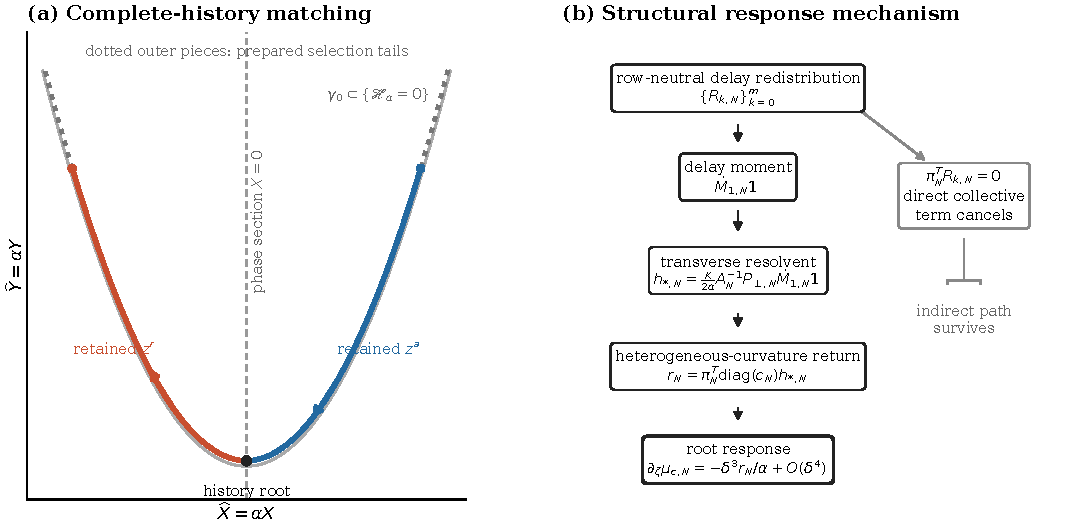
\includegraphics[width=.94\textwidth]{figures/root-mechanism.pdf}
\caption{\textbf{Projection-blind return and the anchored heteroclinic-canard
root.}
\textup{(a)} Schematic history-space projection for one fixed anchored RFDE:
the incoming branch tracks attracting and repelling slow-history graphs and
then enters the intrinsic stable sheet of \(E_N^-\).  The shaded tube is where
the anchored and original equations agree exactly; positions are not
quantitative.  \textup{(b)} Proved information path.  Two separated delays
make the blind source onto, whereas one merged delay gives the leading
first-moment no-go; the returned covector is the root derivative.
\textup{(c)} Schematic root graphs for two anchors.  Absolute roots may differ,
but modelwise centering and \(\delta^{-3}\) scaling give the common tangent
\(\Lambda_N(R)+O(\delta)\) and limiting conormal
\(\mathrm d\xi-\Lambda_N(R)\mathrm d\zeta\).  No root for the unanchored law,
or equality across anchors, is asserted.}
\label{fig:root-mechanism}
\end{figure}


\subsection{Why the global anchor is not a preparation}

The original recovery equation has a genuine obstruction: every equilibrium
lies on the near-fold relation
\(\pi_N^T(v-\mathbf1)=\delta^2\nu\), so it supplies no equilibrium on the
two fixed outer components.  In a homogeneous admissible subclass the
near-fold equilibrium also has a two-dimensional real unstable manifold;
past convergence plus one phase row therefore fails to select a history.
This is proved in \cref{prop:main-original-recovery-anchor-no-go}, rather than
hidden inside a choice of cutoff.

We resolve that obstruction by declaring a different, global model class.
An anchor multiplier \(g_{\rm anc}\) is fixed as part of the recovery law
before any root is sought.  The class is nonempty, bounded in \(C^{12}\), and
has prescribed simple zeros at \(\pm r_A\).  Every member equals one on a
fixed central interval, so the anchored and original RFDEs agree literally as
maps on the full retained depth-two history tube.  Outside that tube the
multiplier creates the two exact hyperbolic equilibria used in
\cref{eq:intro-complete-connection}.  The incoming orbit is the positive-time
image of \(W^u(E_N^+)\); the outgoing object is an intrinsic nonlinear stable
history sheet obtained from a half-line terminal condition at \(+\infty\).
Neither is supplied by a finite terminal row or an ambient backward RFDE
semiflow.

Consequently, for a fixed \(g_{\rm anc}\), the zero in
\cref{eq:intro-physical-root} is a property of one autonomous RFDE and not of
a proof preparation.  Changing \(g_{\rm anc}\) changes the global equation,
so equality of exact roots across anchors would be neither expected nor
geometrically natural.  What survives the entire bounded anchor class is the
modelwise-centered leading conormal.  This distinction is essential: we prove
an intrinsic root for every fixed anchored model and an anchor-robust response
jet, but no maximal canard for the unanchored recovery law.

\subsection{Precise novelty and relation to earlier work}

Classical geometric singular perturbation theory explains planar fold
canards and canard explosions
\citep{krupa2001relaxation,krupa2001extending}.  Delayed canards occur in
machining and FitzHugh--Nagumo-type equations, and infinite-dimensional local
fast--slow theory now covers broad evolution-equation settings
\citep{campbell2009delay,krupa2016complex,krupa2016explosion,%
avitabile2020local,hummel2022slow}.  Canards and canard-mediated transitions
also occur in stochastic, adaptive, consensus, and mean-field networks
\citep{touboul2015noise,ciszak2021collective,jardon2020consensus,%
qin2023tipping,balzer2024cascading}.  We therefore do not claim the first
delayed canard, the first network canard, or a new general theory of
infinite-dimensional slow manifolds.

Invariant-manifold and heteroclinic theory for RFDE semiflows is well
established, as are exponential dichotomies and Lin/Fredholm matching
\citep{hale1986heteroclinic,lin1986exponential,magalhaes1987persistence,%
bates1998invariant,malletparet1999fredholm,hupkes2009lin}.  Connections for
delay equations can also be formulated and computed as projected boundary
value problems with stable and unstable manifold data
\citep{henot2023homoclinic}.  We use these ideas, but do not present the
Banach-space stable-manifold theorem, Lyapunov--Perron method, Fredholm
alternative, or implicit-function theorem as independent novelties.

The projection issue is different from exact lumpability, which requires a
vector field to descend to a closed quotient
\citep{horstmeyer2016lumpability}.  It is also different from structural
unidentifiability, where an entire input--output behavior is invariant under a
parameter change
\citep{bearup2013inputoutput,villaverde2017dynamical}.  Mori--Zwanzig memory
provides a broad precedent for unresolved variables leaving and returning to a
subnetwork
\citep{chorin2002optimal,herrera2018memory,herrera2020tractable}.  Here the
return is resolved explicitly into a delay-moment source, a
Dobrushin-controlled history inverse, and a one-dimensional connection
conormal.  Standard adjoint sensitivity expresses scalar responses as
covector pairings, including for time-lagged systems
\citep{cacuci1981sensitivity,rihan2003sensitivity}; our point is that the
covector remains fully recoverable from a parameter class that is exactly
invisible to the chosen projection.

The new contribution is therefore the following conjunction, not any one of
its standard tools:
\begin{enumerate}[label=\textup{N\arabic*.},leftmargin=3.2em]
\item exact same-full-history projection blindness for delay-layer
redistributions, together with a sharp two-delay range theorem and a
merged-one-delay leading no-go;
\item a dimension-uniform transverse lift and hidden return covector under a
common Dobrushin gap;
\item a fixed-model complete-history heteroclinic canard whose structural
derivative is the same covector, with a uniform nonlinear remainder in the
full dual norm;
\item naturality of the resulting connection conormal and its uniform,
modelwise-centered limit over a declared class of global anchors.
\end{enumerate}
To our knowledge, no result in the cited literature combines these four
properties.  The statement is deliberately narrower than general network
observability or reconstruction
\citep{timme2007revealing,zhang2019reconstruction,pereira2025robust}: the
network skeleton, stationary weights, delay locations, and scalar
coefficients are known, and the recovered object is only the compressed
transverse return covector.  Likewise, the two-delay necessity statement is
confined to stationary-row-neutral pure redistribution and its leading
first-moment source.

\subsection{Proof architecture and reusable interface}

The proof has five load-bearing layers.

\begin{enumerate}[label=\textup{P\arabic*.},leftmargin=3.2em]
\item \emph{Blind source algebra.}  Stationary-row cancellation proves
\cref{eq:intro-blindness}.  A two-atom construction realizes each vector in
\(E_N\) and proves the exact constants in
\cref{eq:intro-sharp-source}; a single merged atom cancels.

\item \emph{Dimension-uniform hidden return.}  Dobrushin contraction gives
the stable transverse inverse without reversing the RFDE semiflow.  The
collective/transverse operator is upper triangular rather than an orthogonal
direct sum; Schur elimination produces \(\Lambda_N\) and the dual recovery
formula \cref{eq:intro-dual-reconstruction}.

\item \emph{Local fold passage.}  An invariant complete-history graph,
event-aligned traces, and a Gaussian cokernel calculation transfer the
transverse source through the fold.  Finite-core selected problems are used
as comparison devices, not as the definition of the final root.

\item \emph{Global history objects.}  The anchor indices select one incoming
past-complete branch and one codimension-one future-asymptotic history sheet.
The latter is built directly on a half-line by a stable-forward and
one-dimensional-unstable-backward Lyapunov--Perron problem.  Forward event
holonomy pulls this sheet to the central section.  A capped-action estimate
shows that admissible finite tails and the intrinsic half-line conormal differ
by \(O(\delta^P)\) for every fixed \(P\).

\item \emph{Exact membership and root transfer.}  A compatible tubular chart
separates the complete normal/history coordinate from one scalar canard
coordinate.  Its stable-sheet membership function has derivative exactly one
in that scalar coordinate.  The zero fiber is therefore precisely
\(W^u(E_N^+)\cap W^s(E_N^-)\).  The local coefficient calculation and the
implicit-function theorem yield \cref{eq:intro-root-jet}; forward-holonomy
pullback proves section and conormal naturality.
\end{enumerate}

This factorization is also a portability checklist.  To use the mechanism in
another RFDE, one must verify: exact blindness on the full history space; a
source map with a controlled right inverse; a transverse history inverse; a
one-dimensional collective return cokernel; genuine incoming and outgoing
complete-history objects; and a weighted \(C^1\) comparison connecting the
local coefficient to their exact membership relation.  The abstract source,
Schur, and root-transfer statements are separated in
\cref{sec:abstract-response} so that these obligations can be checked without
copying the present model.

\subsection{Organization}

\Cref{sec:model-results} defines the shared-resource network and proves the
blind-source dichotomy, dual reconstruction, finite-scale probes, and sparse
examples.  \Cref{sec:abstract-response} isolates the reusable source--Schur--root
interface.  \Cref{sec:network-mechanism} constructs the invariant history
graph and computes the local return coefficient.  The compact
local-to-global interface in \cref{sec:main-outer-interface} records both the
exact original-endpoint passage and the obstruction in the unanchored
recovery law.  \Cref{sec:anchored-physical-connection} constructs the global
anchors, half-line stable sheet, exact membership gap, heteroclinic root, and
intrinsic conormal.  The supplement contains only the preparation, finite-gap,
compressed outer-passage, and half-line proofs needed for that theorem.
